\chapter{Desenvolvimento}
\label{cap:desenvolvimento}

\section{Classificação baseada em templates}
\label{sec:classificador}

    Para reconhecer quais acordes estão sendo tocados numa música a partir de uma gravação, \cite{muller} propõe um algoritmo que se divide em duas partes: extração de características (\textit{features}) e casamento de padrões.

    A primeira consiste na construção, usando a STFT, do cromagrama do sinal. O croma é escolhido como \textit{feature} porque captura informações tonais da música, que compõem sua harmonia, da qual os acordes são elementos. Assim, se define $X = (x_1\textrm{, }x_2\textrm{, }\dots\textrm{, }x_n)$ como sequência de \textit{features}, onde cada elemento $x_i \in R^{12}$ é um croma de uma janela do sinal.

    A segunda etapa do algoritmo consiste em etiquetar cada janela da etapa anterior com um acorde. Para isso, define-se o conjunto $\Lambda$ de acordes a serem levados em consideração durante a classificação. No escopo deste trabalho, tomou-se como $\Lambda$ o conjunto de todas as tríades maiores e menores:

    \begin{equation}\label{Lambda}
        \Lambda = \{
            \textrm{C},
            \textrm{C}\sharp,
            \dots,
            \textrm{A}\sharp,
            \textrm{B},
            \textrm{Cm},
            \textrm{C}\sharp\textrm{m},
            \dots,
            \textrm{A}\sharp\textrm{m},
            \textrm{Bm}
        \}\mbox{.}
    \end{equation}
    
    % Conjunto T de cromas-template dos acordes (bijeção de Lambda)
    Define-se, também, um conjunto $T \subset R^{12}$ de \textit{templates de croma}, de forma que cada acorde considerado na classificação possua um representante no conjunto de templates de croma, ou seja:
    
    \[
      \exists t_\lambda \in T \textrm{, } \forall \lambda \in \Lambda\mbox{.}
    \]
    
    Esse conjunto é construído de forma que cada template se pareça com o croma de uma janela de áudio onde seu respectivo acorde soa. O algoritmo pressupõe que esse conjunto já foi pré-computado.
    
    O conjunto de templates de croma mais simples é o de \textit{templates binários}. Sua construção consiste em definir para cada $\lambda \in \Lambda$ um $t_\lambda \in R^{12}$ tal que:
    
    \[
        {(t_\lambda)}_j = \left\{
            \begin{array}{@{}ll@{}}
                1, & \textrm{se}\ j \in \mbox{classes}(\lambda)\mbox{,} \\
                0, & \textrm{caso contrário}\mbox{,}
            \end{array}\right.
    \]
    
    \noindent onde $\mbox{classes}(\lambda)$ é o conjunto de índices das classes de altura presentes no acorde $\lambda$ na sequência de classes que começa com a classe dó e segue aumentando cada elemento em um semitom até a classe si. Formalmente, se $\lambda$ é a tríade maior construída a partir da classe de altura $n\in\{0,\ldots,11\}$ então $\mbox{classes}(\lambda)=\{n,(n+5)\% 12,(n+7)\% 12\}$, enquanto a tríade menor a partir de $n$ corresponde a $\mbox{classes}(\lambda)=\{n,(n+4)\% 12,(n+7)\% 12\}$.

    Se define, enfim, a correlação entre um croma $x_i$ e um template $t_\lambda$, que é um valor real que mede quão parecidos eles são. Por simplicidade, usamos o produto interno como medida de correlação. É importante que ambos os vetores estejam normalizados, para que se possa comparar correlações entre pares diferentes de vetores:
    
    \[
        C(x_i, t_\lambda) =
            \frac{\langle x_i, t_\lambda \rangle}{||x_i|| \cdot ||t_\lambda||}\mbox{.}
    \]
    
    % Comparação de cada cromagrama x extraído do áudio com cada t em T
    Definidos todos os itens acima, o algoritmo de classificação de acordes baseado em templates é descrito em dois passos:

    \begin{enumerate}
        \item Se extrai a sequência $X$ de cromas do sinal;
        \item Para cada $i = 1, 2, \dots, n$, a i-ésima janela do sinal       é classificada com o acorde $\lambda_i$ definido por:
        
        \[
            \lambda_i = \underset{\lambda \in \Lambda}{\arg \max}\{C(x_i, t_\lambda)\}\mbox{.}
        \]
        
    \end{enumerate}

    O algoritmo apresentado é uma das possíveis soluções para o problema. Porém, alguns fatores limitam a acurácia da sua classificação. Por exemplo: o conjunto $\Lambda$ usado possui apenas 24 acordes, quando o conjunto de todos os acordes existentes é muito maior. Num sinal de áudio que representa uma música, pode haver uma quantidade qualquer de acordes que não estão presentes em $\Lambda$.

    Outro fator que diminui a robustez do algoritmo é o conjunto $T$. Apesar de modelarem com simplicidade os cromas de acordes, os templates binários refletem pouco da realidade, o que será discutido em mais detalhes na seção seguinte.

    Por essas e outras razões, algumas técnicas de aperfeiçoamento do algoritmo foram experimentadas para melhorar sua acurácia. Essas técnicas serão descritas nas subseções seguintes.


    \subsection{Templates aprendidos}
        Templates binários são modelos simples para cromas em que soam determinado acorde. Contudo, num sinal de áudio gravado em uma performance musical do mundo real, nunca se encontrará um croma igual a um template binário.

        O motivo é que nenhum som produzido por instrumentos musicais do mundo real pode ser representado por apenas uma senoide. Em primeiro lugar, sempre haverá a presença de ruído, que, por menos intenso que seja, trará energia a frequências que não pertencem à formação do acorde tocado. Além disso, haverá também a presença dos harmônicos, que agregam energia (em diversos casos, em quantidade considerável) a diferentes frequências do espectro sonoro. Por fim, a própria digitalização do som e extração do cromagrama são processos que pressupõem discretizações e acréscimo de ruídos ao sinal sonoro original.

        Por essas razões, o template binário não é a representação mais fiel para nosso objetivo. Diante disso, uma alternativa natural é que o conjunto de templates seja aprendido a partir de dados previamente anotados (\textit{ground-truth}). Se sabemos previamente quais acordes soam em cada janela temporal de um determinado conjunto de sinais de áudio, podemos agregar os cromas das janelas agrupando-as por acorde e produzir um template para cada acorde que aparece no conjunto analisado.

        Usando esse tipo de abordagem, é esperado que os templates de croma estejam mais próximos de cromas extraídos de sinais sonoros do mundo real, o que melhoraria as correlações obtidas na etapa de casamento de padrões do algoritmo de classificação.

        A forma mais simples de aprender o template para um acorde é calculando a média~simples de cada componente dos cromas cujas janelas estão anotadas com esse acorde. Tomando o conjunto $T_\lambda$ de todos os cromas extraídos dos sinais de áudio cujas janelas estão anotadas com o acorde $\lambda$, podemos definir a j-ésima componente do template médio $t_\lambda^a$ como:

        \[
            (t_\lambda^a)_j = \frac{1}{|T_\lambda|} \sum_{x \in T_\lambda} x_j\mbox{.}
        \]


    \subsection{CQT em vez de STFT}
        As transformadas CQT e DFT possuem efeitos parecidos: ambas transformam a representação de um sinal do domínio do tempo para o de frequências. Por isso, ambas são adequadas para a construção de um cromagrama, mas não igualmente efetivas.

        O domínio de um sinal transformado por uma STFT tem pontos que representam frequências espaçadas linearmente no intervalo de frequências considerado. Isto significa que o número de \textit{bins} entre 20~Hz e 40~Hz será o mesmo que entre 2.000~Hz e 2.020~Hz. No entanto, o intervalo percebido entre uma nota cuja frequência é 20~Hz e outra cuja frequência é 40~Hz é de uma oitava, enquanto no caso seguinte (2.000~Hz e 2.020~Hz), há um intervalo menor que um semitom. Em outras palavras, a STFT proporciona uma resolução variável: menor para notas graves e maior para notas agudas.

        Dependendo da resolução em frequência da STFT, essa propriedade pode fazer com que, para algum conjunto de notas graves, um mesmo \textit{bin} corresponda a mais de uma nota ao mesmo tempo.

        No caso da CQT, a lógica é diferente: um mesmo intervalo musical (digamos, uma oitava, por exemplo) terá a mesma resolução em \textit{bins} independentemente da altura na qual as notas que o definem são tomadas. Em particular, a identificação de notas graves não é penalizada no agrupamento por classes de altura.
        Por essa razão, o uso da CQT em vez da STFT pode aperfeiçoar a classificação de acordes baseada em templates.

    
    \subsection{Compressão espectral logarítmica}
        É comum que determinadas classes de altura presentes num acorde possuam menos energia em seu croma que outras classes ausentes no mesmo. Isso ocorre, por exemplo, devido à grande quantidade de energia que alguns instrumentos produzem em harmônicos das notas do acorde.
        
        Para que a distribuição da energia num croma seja mais uniforme, pode-se aplicar uma técnica conhecida como \textit{compressão espectral}. Essa técnica consiste na aplicação de uma função de compressão $\Gamma_c$ em todos os elementos do croma, onde $c$ é o \textit{fator de compressão}, que é proporcional a quão uniforme será o croma após a compressão. O ganho esperado com essa técnica é a enfatização de classes de altura que possuem pouca energia, porém são perceptíveis na harmonia da música.
        A função de compressão usada, conforme \cite{muller}, foi:

        \[
            (\Gamma_c(x))_i = \log(1 + cx_i)\mbox{.}
        \]

        Encontrar uma constante $c$ adequada é de fundamental importância: valores muito pequenos de $c$ farão com que a compressão não interfira muito no resultado da classificação, enquanto que valores muito grandes descaracterizarão a harmonia presente nos cromas, tornando-o demasiadamente uniformes.

    \subsection{Suavização temporal}
        Em muitos sinais de áudio é comum que, dentro de um período de tempo de algumas janelas em que um mesmo acorde é tocado, hajam variações locais irrelevantes nos cromas.
        Isso pode acontecer por diferentes motivos. Um deles é a presença de ``acordes quebrados'', que são aqueles cujas notas não são tocadas simultaneamente, mas sim uma de cada vez. Por exemplo, um acorde de dó maior (que é formado pelas notas dó, mi e sol) pode ser tocado de forma sequencial, ``arpejando-se'' as três notas que o compõem. Nesse caso, ainda que cada nota continue soando pelas janelas subsequentes à qual foi tocada, é provável que elas contenham menos energia provinda dessa nota e mais das outras.
        
        Variações locais irrelevantes nos cromas podem desencadear, neste algoritmo, variações locais equivocadas na classificação.
        Com essa motivação, uma técnica que pode apresentar melhoria expressiva na acurácia da classificação é a \textit{suavização temporal} dos cromas antes da etapa de casamento de padrões. Essa prática espalha a energia presente em cada nota de um croma para os cromas vizinhos e funciona como um filtro passa-baixas para cada classe de altura da sequência de cromas.
        
        Para se aplicar essa técnica, define-se uma nova sequência de cromas $\hat{X}$ a partir de $X$. O i-ésimo croma de $\hat{X}$ será igual à média (componente a componente) dele com os $L$ cromas vizinhos anteriores e posteriores:
        
        \[
            \begin{split}
                (\hat{x}_i)_j   &= \frac{(x_i)_j + \sum_{k = 1}^L ((x_{i - k})_j + (x_{i + k})_j)}{2L + 1}
            \end{split}\mbox{.}
        \]
        
        Na etapa de casamento de padrões, a sequência de cromas a ser considerada será $\hat{X}$ em vez de $X$.
        
    \subsection{Estimativa de afinação}
        Agrupar a energia do espectrograma de um sinal de áudio por classes de altura envolve, necessariamente, a definição de uma base de afinação: uma frequência de referência para uma nota específica, a partir da qual se calculará a frequência correta de todas as notas.

        Em geral, a afinação utilizada como referência na música ocidental nos dias atuais é a nota chamada \textbf{Lá~4} com frequência 440~Hz. Essa convenção foi definida pela Organização Internacional para Padronização como a norma ISO~16.

        Apesar de ser uma convenção, há exceções em que a afinação em Lá~440 não é utilizada. Num algoritmo de reconhecimento de acordes para uso geral (sem restrição da afinação da música), é importante se saber previamente qual afinação é utilizada, de forma que a construção do cromagrama seja a mais precisa possível.

        Sem pressupor que esse dado é de conhecimento prévio, pode-se utilizar alguma técnica de estimativa de afinação. No contexto deste trabalho utilizou-se interpolação parabólica para fazer essa estimativa, que é o método padrão da biblioteca escolhida (vide Seção~\ref{sec:implementacao}) para processamento de áudio.

    \subsection{Pós-filtragem}
    \label{subsec:pos-filtragem}

        Esta subseção explicará a melhoria que se pode obter acrescentando uma etapa ao algoritmo: após o casamento de padrões, pode-se aplicar a chamada  ``pós-filtragem'', que visa eliminar acordes aparentemente aleatórios que aparecem em algumas classificações entre sequências de acordes iguais. Por exemplo:
        
            \[
                (\dots A, A, A, F\sharp m, A, A, A \dots)\mbox{.}
            \]

        Na classificação apresentada, o acorde F$\sharp$m aparenta ser um erro, pois é improvável que em uma música haja uma troca de acorde que dure apenas o equivalente a uma janela temporal (considerando que as janelas, no escopo deste trabalho, têm, no máximo, perto de dois décimos de segundo).
        
        Uma forma de tentar corrigir esse tipo de erro é construindo uma nova classificação a partir da classificação original. Nesta nova classificação, cada item seria calculado a partir da classificação original através de um voto de maioria que considera o item original e seus vizinhos anteriores e posteriores. É necessário definir quantos vizinhos serão considerados.

\section{Implementação}
\label{sec:implementacao} 
    O objetivo deste trabalho não é a implementação de um sistema de reconhecimento de acordes, mas sim o estudo de um algoritmo que resolve este problema. As escolhas das tecnologias e arquitetura para a implementação do algoritmo observou tal consideração.
    
    A linguagem escolhida para implementação foi Ruby, devido à facilidade para construção de um código-fonte legível e à forte familiaridade do autor com ela.
    
    % TODO citar a librosa da maneira devida (arrumar a entrada dela na bibliografia
    Para as funções clássicas de processamento de áudio - como construção de espectrograma, cromagrama e estimativa de afinação - utilizou-se o \cite{librosa}, um pacote escrito em Python e de simples uso.

    Para a integração do pacote escrito em Python num software escrito em Ruby, utilizou-se a \textit{gem} \href{https://rubygems.org/gems/pycall/versions/1.0.3}{PyCall}\footnote{\url{https://rubygems.org/gems/pycall/versions/1.0.3}}, que possibilitou a adição de uma interface para o Librosa de forma direta.
    
    O \href{https://github.com/gutomotta/chors}{código}\footnote{\url{https://github.com/gutomotta/chors}} foi estruturado de forma que se pudesse rodar experimentos de forma automatizada. Portanto, foi necessário permitir que a seleção das técnicas de aperfeiçoamento do algoritmo fosse feita via passagem de parâmetros.
    
    Para organizar os experimentos, utilizou-se armazenamento de resultados em disco (com identificadores únicos definidos pelos parâmetros) e carregamento preguiçoso dos resultados, de forma que os experimentos rodados alguma vez em uma certa máquina não precisassem ser rodados novamente caso se desejasse rever os resultados.
    
    A geração de gráficos para análise de dados durante os experimentos foi feita com a \textit{gem} \href{https://github.com/topfunky/gruff}{gruff}\footnote{\url{https://github.com/topfunky/gruff}}.

\section{Metodologia de avaliação}

    Numa aplicação prática, deseja-se que o algoritmo seja capaz de reconhecer os acordes tocados num sinal de áudio com a maior acurácia possível. Para isso, é preciso decidir qual versão do algoritmo usar, onde uma versão é o algoritmo básico acrescentado de algum subconjunto das técnicas de aperfeiçoamento descritas na seção \ref{sec:classificador}.
    
    Avaliar uma versão do algoritmo de reconhecimento de acordes significa, em geral, comparar as sequências de acordes produzidas por ele com uma base de anotações de referência - também chamada de \textit{ground-truth} - que é um conjunto de sinais com anotações feitas manualmente do acorde que é tocado em cada janela temporal de cada sinal.
    
    Para que se possa fazer essa comparação, é necessário, além de contar com uma base de anotações de referência, definir um critério de comparação de acordes que, dadas uma classificação feita pelo algoritmo e uma anotação da base de referência, decide se o acorde foi classificado corretamente. É preciso também definir uma (ou mais) medida de avaliação, que atribui um valor à classificação feita em uma música baseada na comparação de todos os acordes classificados com os respectivos acordes de referência. Por fim, pode-se calcular o valor de tal medida para um subconjunto dos sinais da base de anotações de referência, obtendo, assim, uma avaliação de uma versão do algoritmo.

    Nas subseções seguintes serão discutidas as escolhas feitas em relação a esses três elementos: \textit{ground-truth}, \textit{critério de comparação de acordes} e \textit{medidas de avaliação}. Também se discutirá a escolha do subconjunto da base de \textit{ground-truth} no qual são feitas as medidas de avaliação quando o algoritmo envolve algum processo de aprendizado.
    
    \subsection{Ground-truth}
        Para o escopo deste trabalho, utilizou-se a base de anotações de referência apresentada em \cite{harte}, cujos fonogramas (registros sonoros em sinais de áudio) formam a discografia de estúdio da banda The Beatles, que consiste em 180~faixas distribuídas em 13~CDs, com um total de 8~horas, 8~minutos e 53~segundos de áudio.
        
        Os arquivos dessa base seguem o formato .lab (compatível com programas como Sonic Visualiser e Wavesurfer), que é um arquivo de texto ASCII cujas linhas são compostas de três itens separados por espaço:
        
        \begin{center}
            $\langle$início$\rangle$
            $\langle$fim$\rangle$
            $\langle$etiqueta$\rangle$
        \end{center}
        
       \noindent onde \textit{início} e \textit{fim} são números de ponto flutuante que indicam em que momento no tempo (em segundos) o acorde começou e terminou, respectivamente, e \textit{etiqueta} é uma cadeia de caracteres que identifica tal acorde.
        
        As etiquetas seguem uma notação definida detalhadamente em \cite{harte}, onde cada etiqueta possível determina apenas um acorde.


    \subsection{Comparação de acordes}
        Um critério de comparação entre um acorde classificado e um acorde de referência é uma função binária $E: (\Lambda, \hat{\Lambda}) \rightarrow \{0, 1\}$, onde $\hat{\Lambda}$ é o conjunto de todos os acordes existentes e $\Lambda \subset \hat{\Lambda}$ é o conjunto definido na Equação \ref{Lambda}. Dizemos que um acorde $\lambda_i$ \textit{passou} no critério de comparação com~$\hat{\lambda}_i$ se $E(\lambda_i, \hat{\lambda}_i) = 1$, onde $\hat{\lambda}_i$ é o respectivo acorde da base de anotações de referência.
        
        Um possível critério é aquele em que $E(\lambda_i, \hat{\lambda}_i) = 1 \Leftrightarrow \mbox{classes}(\lambda_i) = \mbox{classes}(\hat{\lambda}_i)$. Este critério é intuitivamente válido, porém, se $\Lambda$ não é muito grande, ele pode não capturar casos em que gostaríamos de considerar a classificação correta.
        
        Tomemos como exemplo o acorde Am7 $\notin \Lambda$. Se Am7 é o acorde de referência para uma janela de sinal e o algoritmo classificar tal janela com Am $\in \Lambda$, se poderia considerar essa classificação como um acerto, já que esses acordes são iguais exceto por uma nota acrescentada (sol) em Am7. De fato, isso poderia se aplicar a todos os acordes que são tríades com notas acrescentadas.
        
        Por essa razão, o critério de comparação de acordes escolhido foi $E_0$ tal que:
        \[
            E_0(\lambda_i, \hat{\lambda}_i) = 1 \Leftrightarrow \mbox{classes}(\lambda_i) \subseteq \mbox{classes}(\hat{\lambda}_i)\mbox{.}
        \]
        
        Essa escolha tem ainda outras consequências que valem atenção. Em alguns casos, acordes possuem um conjunto de classes de altura que são subconjuntos do de outros acordes cujas tônicas não são a mesma. Um exemplo desse caso são os acordes G $\in \Lambda$ e Em7 $\notin \Lambda$. Se observa que $\mbox{classes}(Em7) = \{ 2, 4, 7, 11 \}$ e $\mbox{classes}(G) = \{ 2, 7, 11 \}$, e, por isso, $\mbox{classes}(G)~\subset~\mbox{classes}(Em7)$, o que configura um acerto no critério $E_0$. No entanto a tônica de G é a nota sol, enquanto que a tônica de Em7 é a nota mi.
        
        Essa consequência de $E_0$ não foi considerada como inadequada no escopo deste trabalho. A condição $\mbox{classes}(\lambda_i) \subseteq \mbox{classes}(\hat{\lambda_i})$ é suficiente para que ambos acordes possuam certa semelhança sonora. Considerando o conjunto $\Lambda$ escolhido, é necessário certa tolerância em relação à consideração de acertos, para que se possa obter números efetivamente comparáveis quando se experimente uma técnica de aperfeiçoamento do algoritmo.
        
    
    \subsection{Precisão}
        É chamado de \textit{classificação} o resultado do algoritmo para algum sinal específico. Um \textit{verdadeiro positivo} é uma janela de uma classificação cujo acorde classificado passou no critério de comparação com o respectivo acorde da base de anotações de referência. Por sua vez, é chamada de \textit{falso positivo} a janela cujo acorde classificado, analogamente, \textit{não passou} no critério de comparação.
        
        Na base de anotações de referência, algumas janelas são marcadas como \textit{sem acorde}. Isso acontece quando o trecho de áudio não possui conteúdo harmônico significativo (por exemplo, em um solo de bateria ou em um trecho onde só se podem ouvir aplausos). Janelas sem acorde foram descartadas nas avaliações feitas nos experimentos deste trabalho.
        
        Definem-se os conjuntos \textit{VP} e \textit{FP} de todos os verdadeiros positivos e falsos positivos, respectivamente, de uma classificação. Então, a precisão $P$ de uma classificação é calculada da seguinte maneira:
        
        \[
            P = \frac{\#VP}{\#VP + \#FP}.
        \]
        
        O cálculo da precisão poderia, alternativamente, atribuir um peso a cada verdadeiro positivo e falso positivo proporcionais à duração de suas respectivas janelas, somando os pesos dos verdadeiros positivos e finalmente dividindo pela duração total do sinal. No contexto deste trabalho, as janelas têm duração fixa e, por isso, não se utilizaram pesos distintos.
    
    \subsection{Validação cruzada K-fold}
        Algumas versões do algoritmo de classificação de acordes baseada em templates podem depender de um processo de aprendizado. Por exemplo, quando se utilizam templates aprendidos em vez de binários, é necessário que algum subconjunto da base de \textit{ground-truth} seja usado para a computação dos templates.
        
        Nesses casos, é necessária atenção no momento de avaliar o algoritmo. Se levarmos em consideração a precisão da classificação de músicas que foram usadas no processo de aprendizado dos acordes, teremos uma situação conhecida no contexto de aprendizagem computacional como \textit{overlapping}. Avaliações com \textit{overlapping} não podem ser consideradas válidas, pois utilizam dados iguais para construção e validação do algoritmo.
        
        Uma possibilidade para a avaliação de tais versões é o uso de um processo chamado \textit{k-fold cross validation} ou \textit{validação cruzada k-fold}. Ele consiste na divisão da base de \textit{ground-truth} em $k$ partes iguais (ou \textit{dobras}), aleatoriamente. O processo de avaliação é feito $k$ vezes, cada uma delas usando uma das dobras como conjunto de validação (e as outras $k - 1$ como conjunto de aprendizagem).
        
        Quando avaliada dessa forma, uma versão do algoritmo terá na verdade $k$ avaliações. No experimentos realizados neste trabalho, sendo necessária a produção de uma avaliação única, tomou-se sempre a média simples das $k$ avaliações.


\section{Experimentos}

    Esta seção descreve os experimentos feitos para analisar os resultados das diferentes versões do algoritmo de classificação de acordes baseada em templates, procurando justificar as eficácias obtidas em cada versão.
    
    Como são muitas as técnicas de aperfeiçoamento do algoritmo, foi necessário implementá-lo de uma forma geral, que permitisse a definição da versão através de passagem de parâmetros, além de um esquema de armazenamento de resultados que permitisse fácil identificação e comparação de resultados.
    
    Os experimentos foram feitos seguindo este esquema:
    
    \begin{enumerate}
        \item Definição de uma versão do algoritmo;
        \item Construção dos templates para essa versão;
        \item Classificação das faixas no(s) conjunto(s) de fonogramas de validação;
        \item Avaliação das classificações (cálculo de precisão);
        \item Avaliação da versão (definida como média das precisões das classificações);
        \item Análise de resultados.
    \end{enumerate}
    
    A etapa de análise de resultados consistiu na comparação da avaliação entre diferentes versões e na verificação de precisões específicas dentro do conjunto de precisões obtido. Para comparar versões entre si, se calculou a média das precisões obtidas e, em alguns casos, se observou a distribuição das precisões. Em todas as versões analisadas, a distribuição das precisões obtidas nos experimentos não foi uniforme - o que seria desejável, pois traria uma maior previsibilidade quanto à qualidade do reconhecimento do algoritmo de forma geral. Além disso, se observaram ocorrências de precisões muito próximas de zero.
    
    Nas subseções seguintes, são descritas análises de como as técnicas de aperfeiçoamento influenciaram na alteração dos resultados. Os experimentos, por padrão, foram feitos com uma taxa de amostragem de 22.050~Hz, janelas de 4096 amostras e saltos entre janelas de 2048 amostras.
    
    \subsection{Estimativa de afinação}
    
        Conforme explicado anteriormente, a extração do cromagrama de um sinal de áudio pressupõe o uso de um valor de frequência como referência de afinação da nota Lá~4. A qualidade do cromagrama obtido do sinal é impactada pelo valor de afinação utilizado como referência.
        
        Nos experimentos feitos, observou-se casos em que a precisão obtida no reconhecimento de acordes foi muito próxima de zero. Um caso particular de resultado pouco satisfatório foi o da canção Lovely Rita, que, no fonograma processado, está afinada com Lá~4 em 425~Hz.
        Tal afinação fez com que a maioria das janelas fosse classificada com acordes um semitom abaixo dos corretos, em todas as versões do algoritmo testadas.
        
        Num experimento isolado, com uso de CQT para extração de cromagramas, foi possível obter uma precisão de ${31.63}\%$ utilizando a afinação correta como base da extração de cromas. Utilizando a afinação estimada, obteve-se uma precisão de apenas ${0.5}\%$.
        
        Em outros casos de afinação desviada, este cenário não se repetiu. Por exemplo, na canção Wild Honey Pie, cujo fonograma teve sua afinação estimada de Lá~4 em aproximadamente 426~Hz \citep[ver][tabela 9.8]{harte}, se obteve uma classificação com precisão de ${14.66}\%$ utilizando algoritmo de estimativa de afinação, contra ${14.39}\%$ com a afinação fornecida como parâmetro. Neste caso, se observou que a estimativa algorítmica da afinação foi mais precisa que a estimativa manual.
    
    \subsection{Transformadas para extração do cromagrama}
    
        Nos experimentos deste trabalho, foram testados dois tipos de transformada na construção de cromagramas: STFT e CQT.
        
        Conforme esperado, os resultados obtidos com a transformada Q-constante foram melhores, mas não muito significativamente, devido ao tamanho da janela usado (4096), que fez com que a resolução da STFT para notas graves não fosse tão baixa. Num primeiro momento, considerando apenas classificações com uso de templates de croma binários, a precisão média obtida com uso de STFT foi de ${32.89}\%$, contra ${34.28}\%$ com uso de CQT.
        
        \begin{figure}[htb]
            \begin{center}
                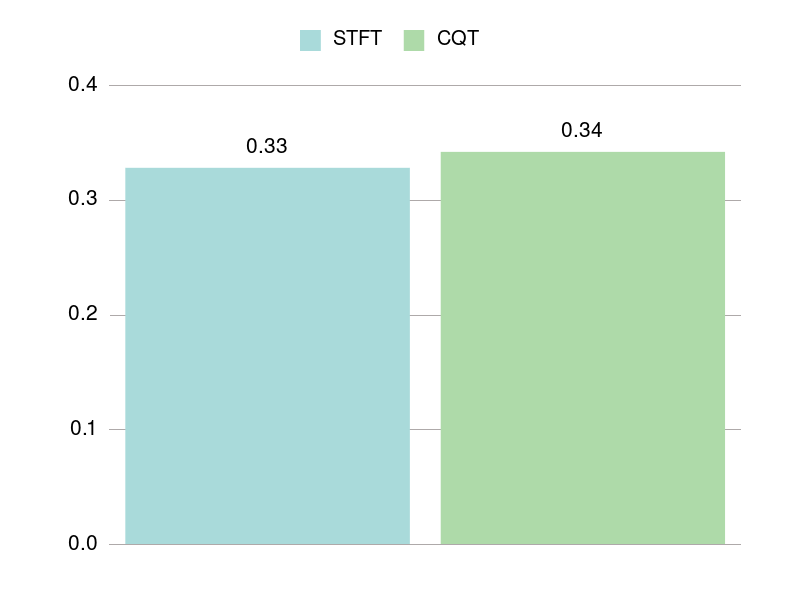
\includegraphics[width=12cm]{figuras/02-stft-e-cqt-com-templates-binarios.png}
                \caption{\label{fig:exp:chroma}Precisões médias obtidas com uso de STFT e CQT para construção do cromagrama.}
            \end{center}
        \end{figure}
        
        Os desvios-padrão obtidos em ambos os casos foram próximos, porém, com uso da CQT, o valor foi ligeiramente menor, o que indica que uma previsibilidade um pouco maior nesse caso. Os resultados completos podem ser vistos na tabela \ref{tabela:stft-vs-cqt}.
    
        \begin{table}[h]
        \centering
        \begin{tabular}{|l|l|l|}
            \hline
    
            \textbf{Transformada} & \textbf{Média} & \textbf{Desvio Padrão} \\
    
            \hline
    
            STFT  & ${32.89}\%$ & ${10.95}\%$ \\
            \textbf{CQT}   & $\textbf{{34.28}\%}$ & $\textbf{{10.12}\%}$
  \\
    
            \hline
        \end{tabular}
        \caption{Comparação das precisões obtidas com uso de duas transformadas diferentes na extração de cromagramas.}
        \label{tabela:stft-vs-cqt}
        \end{table}
    
    \subsection{Templates binários e templates aprendidos}
    
        Devido ao fato de que templates de croma binários não refletem as intensidades reais da distribuição de energia em classes de altura de acordes, espera-se, intuitivamente, que existam templates mais adequados para o reconhecimento de acordes.
        
        No entanto, experimentalmente, se observou que a técnica apresentada de aprendizado de templates - a partir do cálculo da média dos cromas de janelas de áudio previamente rotuladas - não trouxe melhoria nas precisões obtidas.

        \begin{figure}[h]
            \begin{center}
                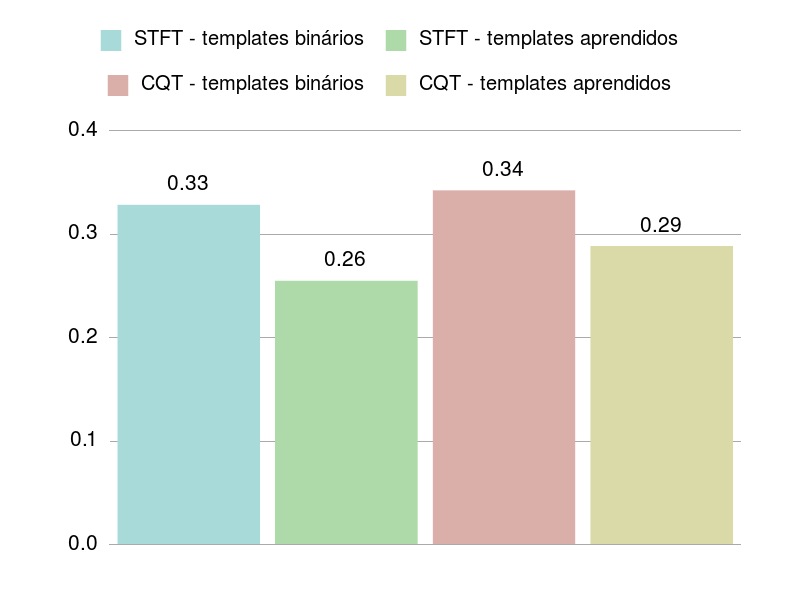
\includegraphics[width=9cm]{figuras/03-stft-e-cqt-templates-bin-e-aprendidos.png}
                \caption{\label{fig:exp:templates_chroma}Comparação entre a precisão média obtida com templates binários e aprendidos.}
            \end{center}
        \end{figure}
        
        Uma possível explicação para tal fato seria um erro de estimativa de afinação dos áudios (leva-se em conta que não se possui uma base de anotações de referência das afinações de cada áudio utilizado nos experimentos). Isso implicaria no agrupamento de cromas que foram extraídos com desvios de afinação e na consequente obtenção de um template médio de má qualidade.
        
        \begin{figure}[h]
        \begin{center}
            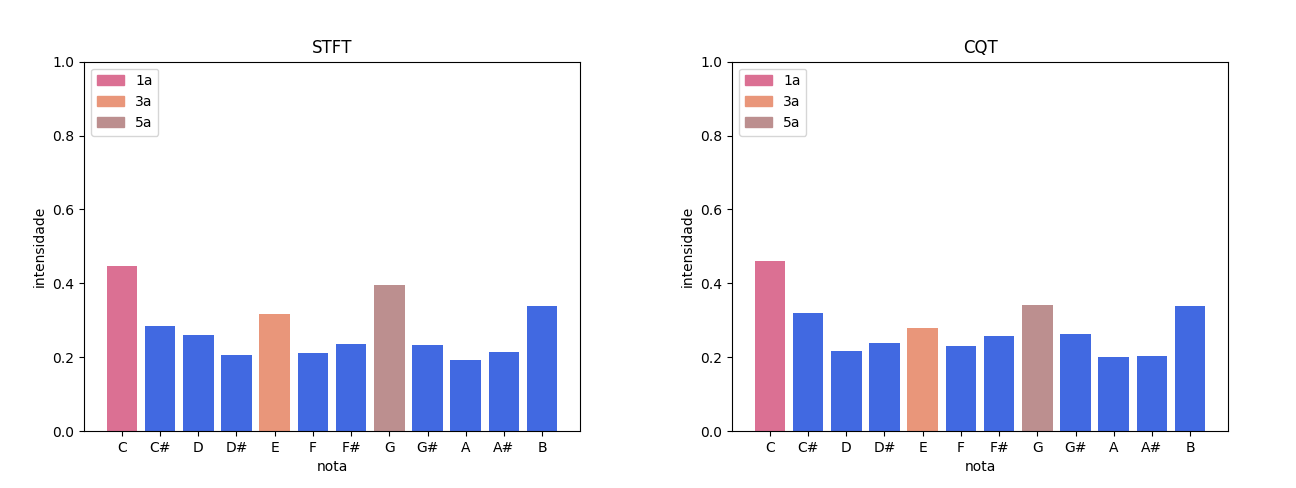
\includegraphics[width=16cm]{figuras/mayor_C.png}   
            \caption{\label{fig:exp:template_c}Visualização do cromagrama template construído a partir de cromas STFT e CQT do acorde \textbf{dó maior} (C). As classes de altura destacadas com cores diferentes refletem as notas presentes no acorde. Nota-se que algumas classes ausentes no acorde (como B, harmônico tanto de G quanto de E) possuem mais energia que outras presentes.}
        \end{center}
        \end{figure}
        
        Na figura \ref{fig:exp:template_c}, pode-se visualizar dois dos templates de croma do acorde dó maior, calculados através da técnica de aprendizado descrita. Três quartos da base de anotações de referência foram usados para o treinamento, e um quarto para a validação.
        
        Nessa figura, percebe-se que as classes de altura de notas que fazem parte da formação do acorde (C, E e G) estão entre as que mais possuem energia no template produzido. Contudo, a intensidade de outras classes de altura, que não fazem parte do acorde mas pertencem aos harmônicos das notas do acorde, também são consideravelmente altas.
        
        Na versão do algoritmo que faz uso de STFT, nota-se uma maior ênfase das classes destacadas, notando-se apenas uma classe (B) com intensidade próxima à de uma classe destacada (C). No versão de CQT, a distribuição da energia é mais uniforme, e diversas classes possuem energia próxima à presente nas classes destacadas, em especial E e G.

        Tanto com STFT como CQT, os resultados pioraram quando se passou do uso de templates binários para o de templates aprendidos. Os resultados estão expostos na tabela \ref{tabela:bin-vs-learn}.


        \begin{table}[h]
        \centering
        \begin{tabular}{|l|l|l|l|}
            \hline
        
            \textbf{Transformada} & \textbf{Templates} & \textbf{Média} & \textbf{Desvio Padrão} \\
        
            \hline

            STFT  & \textbf{binários}   & $\textbf{{32.89}\%}$ & ${10.95}\%$  \\
            STFT  & aprendidos & ${25.55}\%$ & ${8.87}\%$ \\

            \hline

            CQT   & \textbf{binários}   & $\textbf{{34.28}\%}$ & ${10.12}\%$ \\
            CQT   & aprendidos & ${28.89}\%$ & ${10.3}\%$  \\
        
        
            \hline
        \end{tabular}
        \caption{Resultados dos experimentos que usam templates binários contra templates aprendidos na etapa de casamento de padrões.}
        \label{tabela:bin-vs-learn}
        \end{table}
    
    \subsection{Suavização temporal e pós-filtragem}
    
        A suavização temporal é uma técnica de aperfeiçoamento que tem como intenção a captura de harmonias cujos componentes soam ao longo de várias janelas e não necessariamente de forma simultânea. Além disso, se supõe que tal técnica mitigue erros de classificação que ocorrem em janelas isoladas, onde as janelas vizinhas são classificadas corretamente.
        
        Conforme explicado anteriormente, a suavização temporal possui um parâmetro $L$ que corresponde ao número de vizinhos (posteriores e anteriores) usados na suavização. Experi\-mentou-se diversos valores distintos de $L$, e se observou que a melhoria gerada chega a um ponto ótimo, e depois as precisões voltam a cair. Intuitivamente, utilizar um número muito grande de janelas no cálculo dos cromas suavizados aumenta o risco de misturar o conteúdo de cromas que capturam o conteúdo harmônico de dois ou mais acordes, e consequentemente a probabilidade de erro.
        
        O gráfico da figura \ref{fig:exp:suav-temporal} mostra a evolução das precisões médias obtidas com diferentes valores de $L$, comparando os resultados do uso das transformadas STFT e CQT.
        
        \begin{figure}[h]
            \begin{center}
                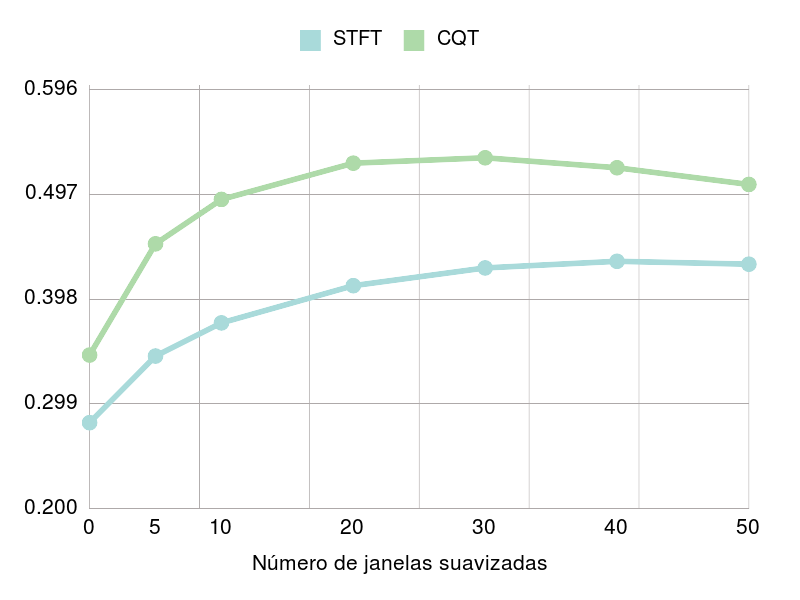
\includegraphics[width=13cm]{figuras/04-stft-e-cqt-bin-suavizacao-temporal.png}
                \caption{\label{fig:exp:suav-temporal}Impacto da suavização temporal com diferentes parâmetros.}
            \end{center}
        \end{figure}
        
        Com a taxa de amostragem e tamanho de janela usados, cada janela temporal tem aproximadamente 180~ms. Os valores ótimos, em função do parâmetro $L$, observados nos experimentos, ocorreram para $L = 10$, o que implica que o número total de janelas suavizadas é 21, o que equivale a aproximadamente ${3.9}~s$ de áudio.
        
        É importante notar que os fonogramas usados nos experimentos são todos de uma mesma banda e que, ainda que sejam bastante diversos, o valor ótimo de $L$ pode ser distinto em outros contextos; vale, no entanto, como uma estimativa.
        
        A tabela \ref{tabela:temp-var-l} traz a precisão média observada para distintos valores de $L$, considerando o uso de STFT e CQT.

        \begin{table}[h]
        \centering
        \begin{tabular}{|l|l|l|}
            \hline
        
            \textbf{Valores de L} & \textbf{Precisão Média STFT} & \textbf{Precisão Média CQT}\\
        
            \hline
        
            0  & ${32.89}\%$           & ${34.28}\%$          \\
            5  & ${45.19}\%$           & ${51.96}\%$           \\
            \textbf{10} & $\textbf{{47.22}\%}$  & $\textbf{{52.0}\%}$          \\
            15 & ${46.02}\%$           & ${48.93}\%$ \\
            20 & ${44.18}\%$           & ${45.5}\%$          \\
            25 & ${42.34}\%$           & ${42.39}\%$          \\
            
            \hline
        \end{tabular}
        \caption{Resultados dos experimentos com templates binários, uso de STFT e CQT e distintos valores do parâmetro $L$ para suavização temporal.}
        \label{tabela:temp-var-l}
        \end{table}

        Os experimentos feitos neste trabalho mostraram que a pós-filtragem conforme definida na subseção \ref{subsec:pos-filtragem} traz certa melhoria na classificação. No entanto, essa melhoria não se acumula com a melhoria trazida pela técnica de suavização temporal. Isso se dá porque a aleatoriedade com que os acordes aparecem numa classificação diminui consideravelmente quando se aplica previamente uma suavização temporal nos cromas.

    \subsection{Compressão espectral}
        
        Durante a experimentação da técnica de compressão espectral logarítmica, se voltou a comparar templates aprendidos e binários. Essa comparação foi motivada pelos resultados expostos em \cite{muller}, figura 5.22, que sugerem que a melhoria no reconhecimento trazida pelo uso de templates aprendidos se apresenta apenas quando combinado com o uso de compressão de cromas.
        
        Dessa forma, os experimentos desta técnica foram divididos em duas etapas: uma fazendo uso de templates binários, e outra, de templates aprendidos.
        
        Os resultados obtidos com uso de templates binários não foram melhorados quando combinados com a etapa de compressão espectral logarítmica. Tal resultado era esperado, pois ao aumentar-se a compressão dos cromas extraídos do sinal de áudio, eles estarão cada vez mais próximos de um croma uniforme, e, portanto, menos similares aos templates binários.
        
        No gráfico da figura \ref{fig:exp:bin-compressao}, observa-se essa tendência. Ainda que haja uma pequena variação positiva da precisão obtida pelo algoritmo quando se usa STFT com compressão, essa variação é inexpressiva - de aproximadamente ${0.25}\%$ no melhor caso (ou seja, com fator de compressão 5). Analogamente, pode-se dizer que as variações negativas trazidas pelo aumento do fator de compressão também são inexpressivas, o que indica uma provável injustificabilidade do uso de tal técnica (que possui um custo computacional) combinado ao de templates binários.
        
        \begin{figure}[h]
            \begin{center}
                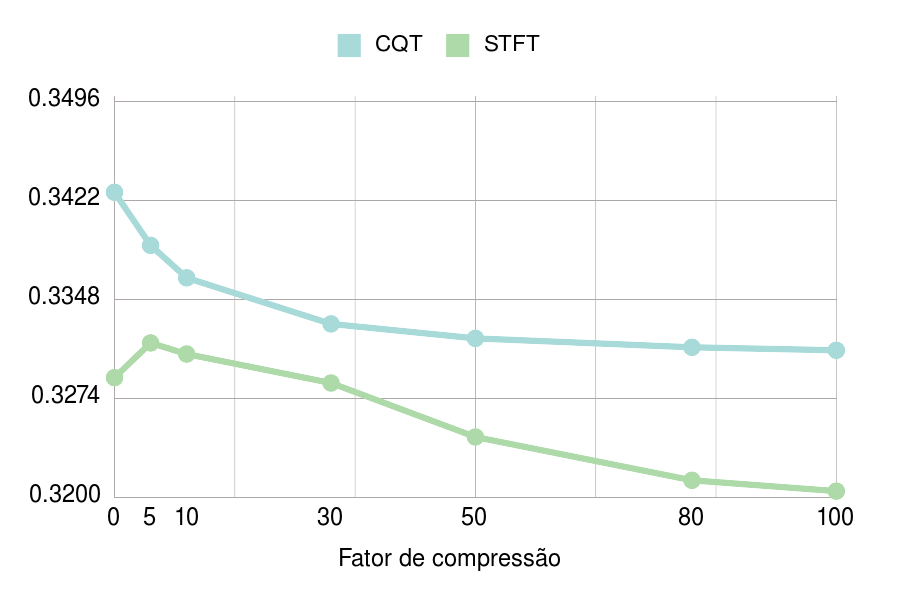
\includegraphics[width=13cm]{figuras/bin-compressao.png}
                \caption{\label{fig:exp:bin-compressao}Efeito da compressão espectral logarítmica nas versões do algoritmo que usam templates binários. Não se observou ganho obtido por esta técnica nestes casos.}
            \end{center}
        \end{figure}
        
        No caso de templates aprendidos com CQT, não se observou uma tendência consistentemente positiva nos resultados obtidos com uso de compressão espectral. Em realidade, o impacto causado pela compressão nesse caso foi bastante pouco significativo.
        
        Já no caso de templates aprendidos com STFT, houve uma melhoria consistente, que chega num ápice com fator de compressão igual a 30 e diminui um pouco com fatores maiores. Tal efeito pode ser observado na figura \ref{fig:exp:cqt-stft-learn-compressao}.
        
        \begin{figure}[h]
            \begin{center}
                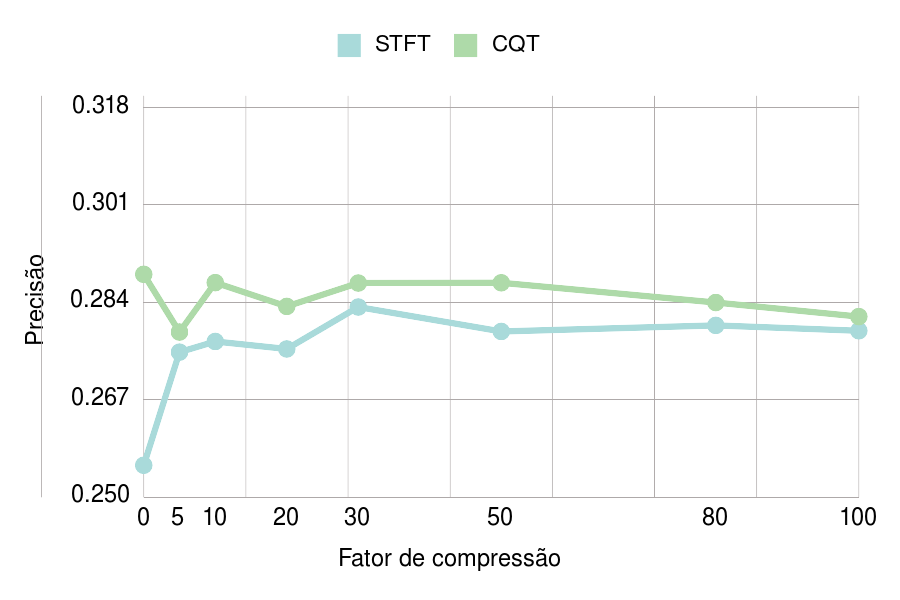
\includegraphics[width=12.5cm]{figuras/11-cqt-stft-learn-compressao.png}
                \caption{\label{fig:exp:cqt-stft-learn-compressao}Efeito da compressão espectral logarítmica nas versões do algoritmo que usam templates aprendidos. Note que o impacto da compressão é pouco significativo quando combinada uso de CQT, porém positivo quando combinada ao uso de STFT.}
            \end{center}
        \end{figure}

        Também se observou que a consistente melhoria trazida pela compressão quando combinada com templates aprendidos e STFT persiste quando é aplicada, posteriormente, a suavização temporal de cromas. No entanto, ainda que a compressão logarítmica melhore os resultados obtidos com uso de templates aprendidos, não foi possível superar os resultados dos templates binários (que, conforme mostrado anteriormente, não se beneficiam do uso de compressão). O gráfico \ref{fig:exp:stft-learn-bin-compressao-smooth} expõe tais resultados.
        
        \begin{figure}[h]
            \begin{center}
                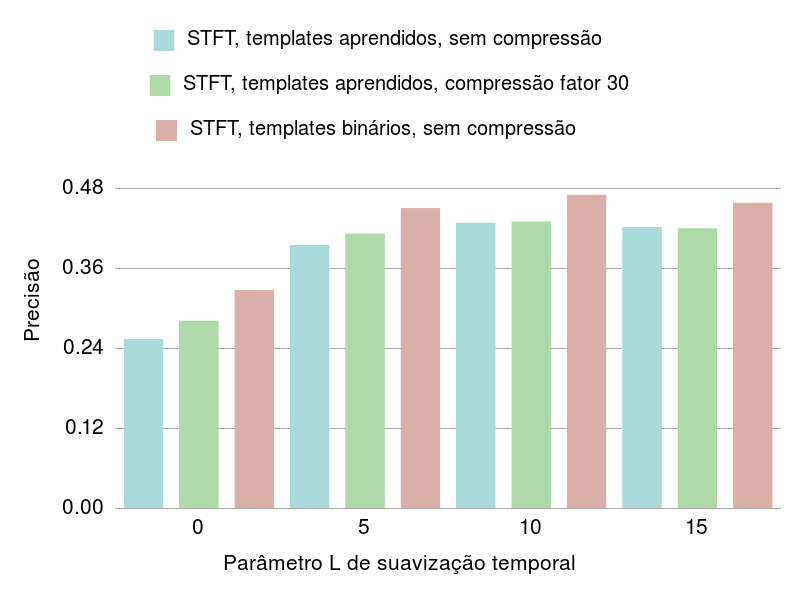
\includegraphics[width=13cm]{figuras/13-stft-learn-bin-compressao-smooth.png}
                \caption{\label{fig:exp:stft-learn-bin-compressao-smooth}Comparação entre as precisões obtidas em três cenários distintos que usam STFT: i) uso de templates aprendidos, sem compressão logarítmica; ii) uso de templates aprendidos, com compressão logarítmica (fator de compressão 30) e iii) uso de templates binários, sem compressão logarítmica. Os três cenários foram testados combinados com suavizações temporais com quatro valores diferentes para o parâmetro L: 0, 5, 10 e 15. Notou-se que a compressão beneficia os resultados obtidos com uso de STFT e templates aprendidos, mas não é suficiente para superar os resultados obtidos com templates binários.}
            \end{center}
        \end{figure}
